\documentclass[twosides, 11pt]{book} 
%\usepackage[utf8]{inputenc} % Required for inputting international characters
\usepackage[T1]{fontenc} % Output font encoding for international characters
\usepackage{cuisine}

\definecolor{cream}{rgb}{1.0, 0.99, 0.82}

\AddToShipoutPictureBG*{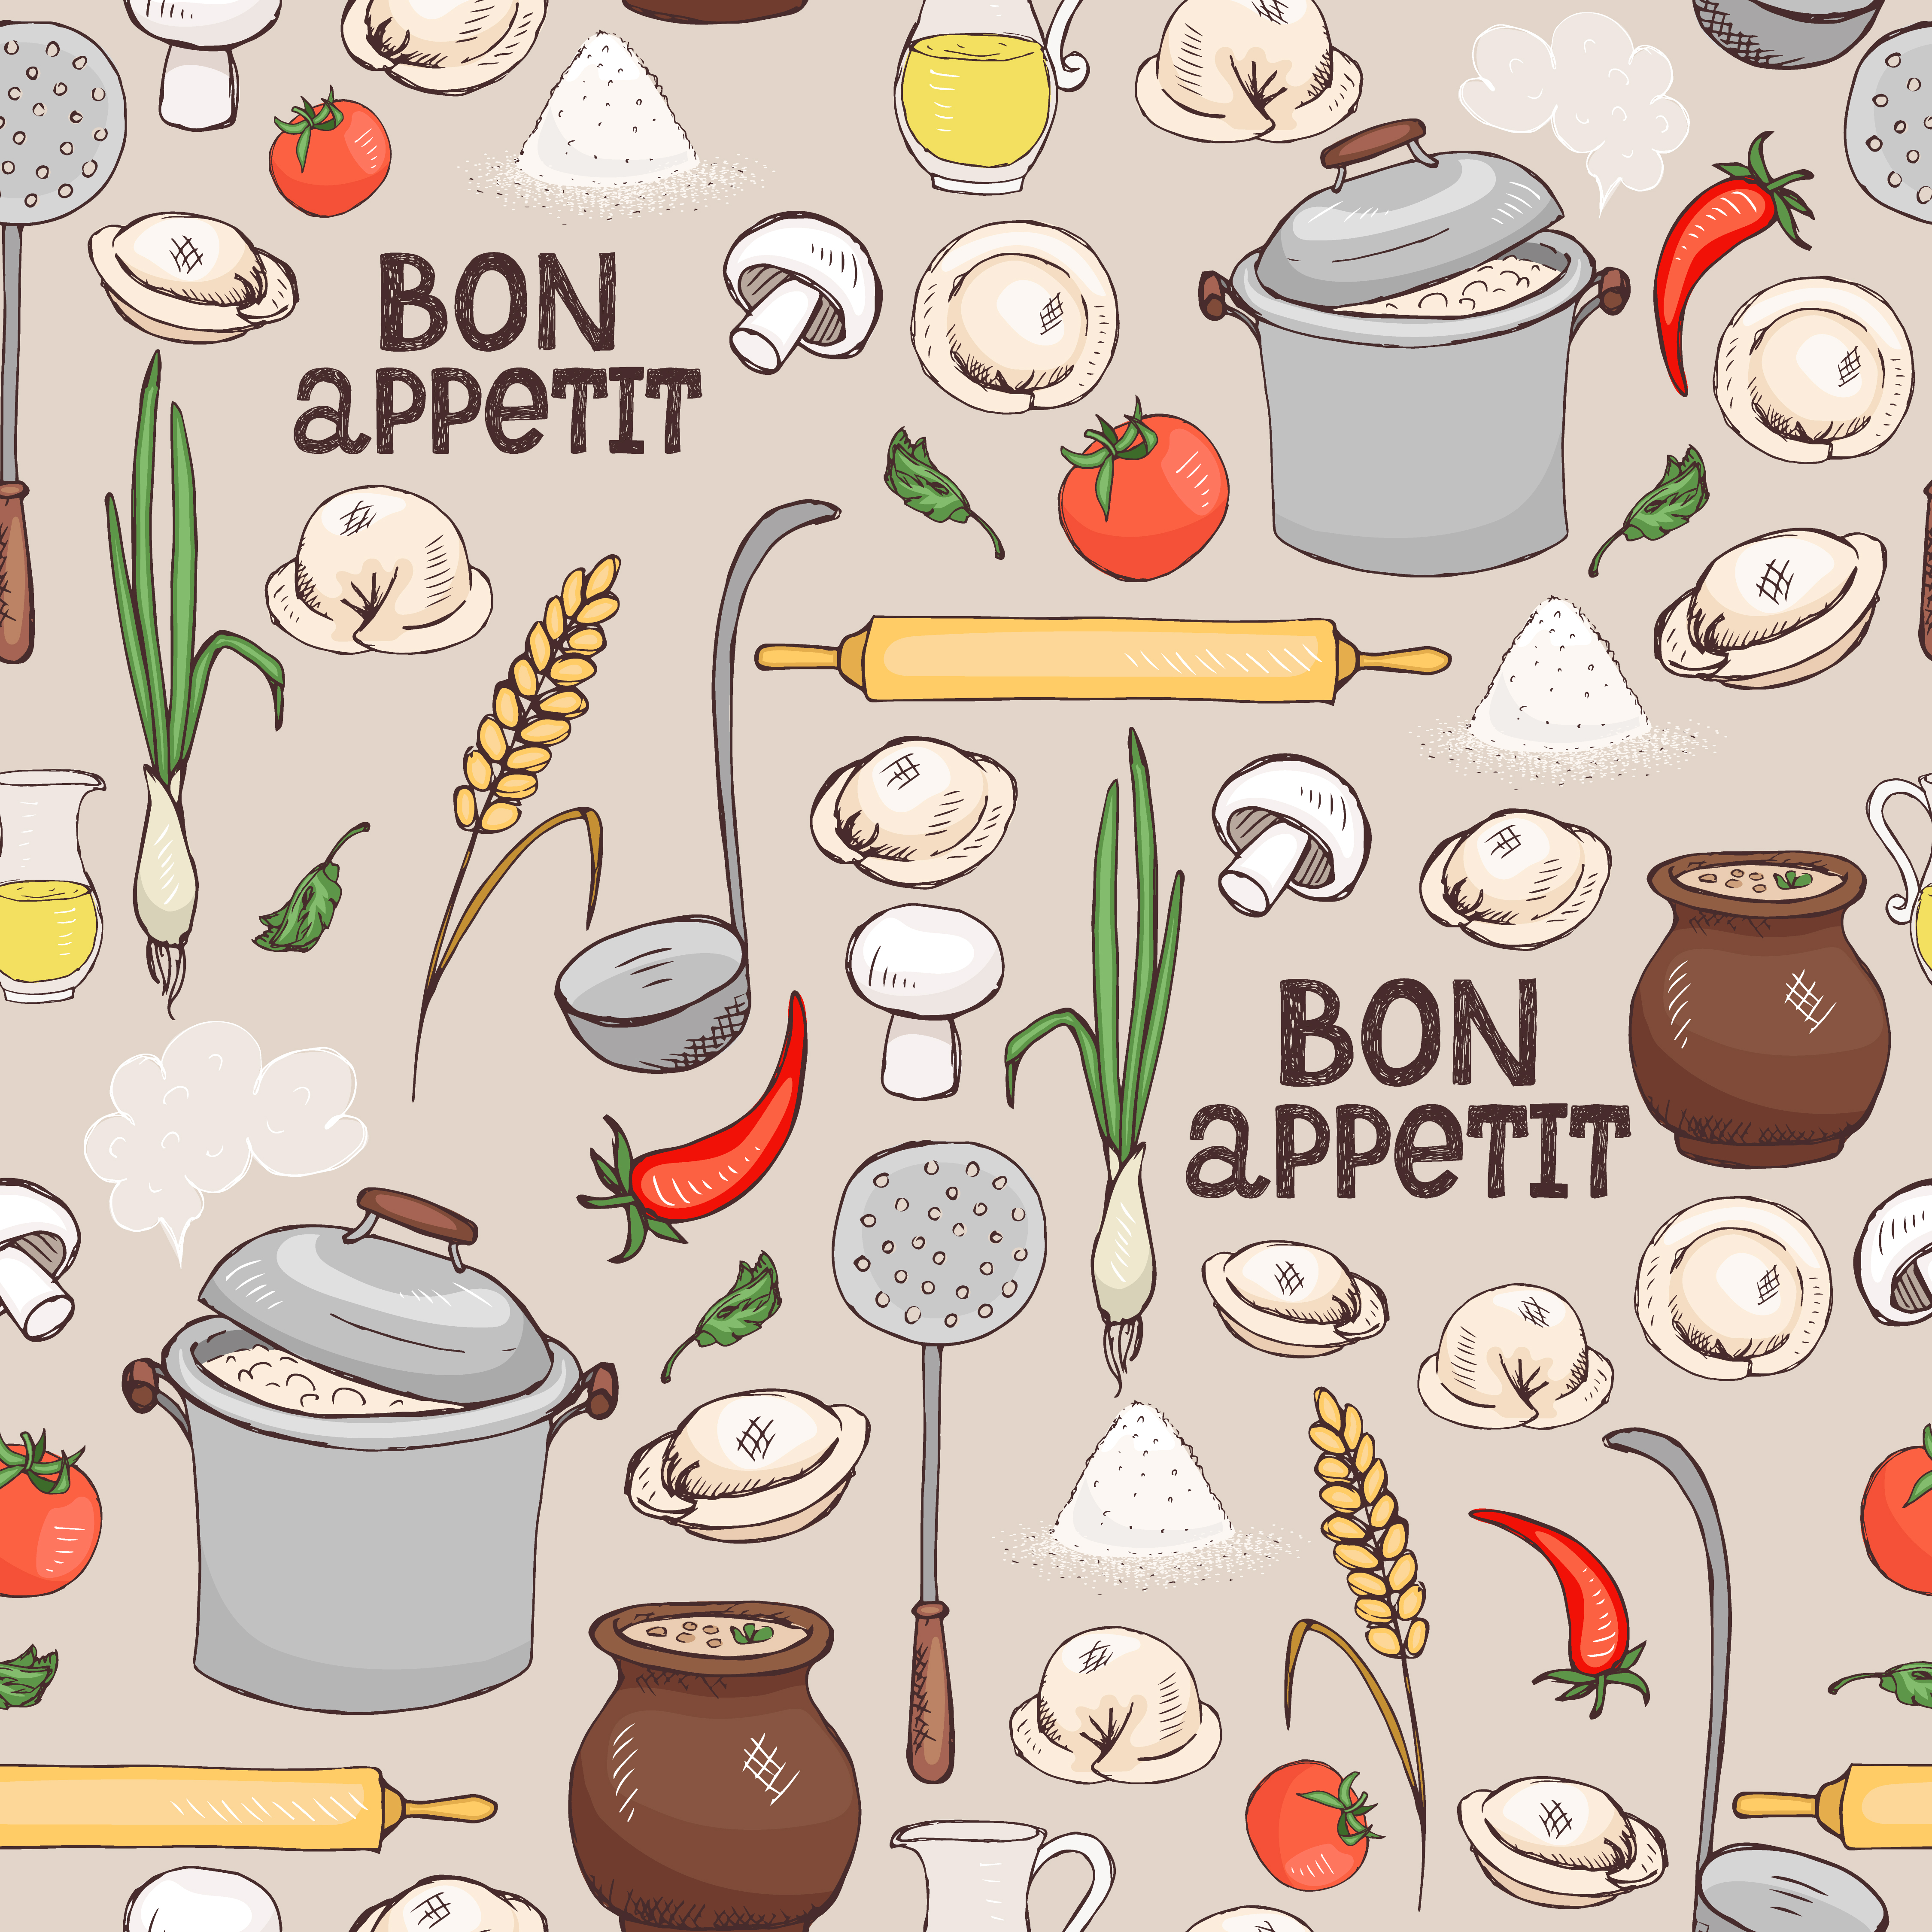
\includegraphics[width=\paperwidth,height=\paperheight]{Pictures/ico/44086.jpg}}

\title{\colorbox{white}{\Huge \bf Recetas de Yorshi}}
\author{\colorbox{white}{\LARGE Jorge Luis Briseño Gómez}}
\date{\colorbox{white}{\large \today}}




\makeindex
\begin{document}
%\doublespacing
%\input{Recipes/Sample}

\maketitle
\tableofcontents
\pagecolor{white!70!cream}

\chapter{Masa Madre}
\begin{spacing}{2.0}
La masa madre es mucho más que un simple ingrediente; es un organismo vivo, una danza de levaduras y bacterias salvajes que se entrelazan para crear panes de un sabor y textura inigualables. Cada burbuja que se forma en su fermentación es una historia de transformación, una prueba del poder de la naturaleza y la paciencia del panadero. A través de este capítulo, exploraremos el fascinante mundo de la masa madre, desde sus orígenes hasta las técnicas más avanzadas para crear panes artesanales que deleitarán hasta al paladar más exigente.
\end{spacing}
%
%       PAN DE MASA MADRE
%
\recette{Pan de Masa Madre}

\preptime{45 min} \cooktime{250\textdegree C, 20 min} \baketime{220\textdegree C, 30 min} \cooltime{60 min} \people{10}

\recipe{
        \unit[400]{g} & Harina panadera\\
        \unit[260]{g} & Agua \\
        \unit[80]{g} & Masa Madre \\
        \unit[8]{g} & Sal 
}{
    \item Mezcla 10g de masa madre con 30g de agua y 40g de harina (proporción 1:3:4).
    \item Combina la masa madre activada con toda el agua y la harina. Deja reposar sin amasar durante 1 hora.
\item Incorpora la sal disuelta en un poco de agua a la masa.
\item Realiza pliegues cada 30 minutos durante las primeras 2 horas. Deja fermentar hasta que la masa aumente un 50-70%.
\item Dale forma a la masa y colócala en un banetón enharinado. Reposa en frío durante 24 horas.
\item Precalienta el horno y hornea el pan. Los primeros 20 min, añade humedad para ayudar al pan a que se expanda. Los últimos 30 min, retira la humedad para obtener una corteza crujiente.
}

\info{Esta receta es para un pan al 65\% de hidratación. Se puede cambiar la hidratación, modificando la cantidad de agua. También se puede modificar la proporción para activar la masa madre a 1:2:2 o 1:3:3, para modificar el sabor y acidez.}
\photo{1-MasaMadre/pan-masa-madre}
%\recette{Pan de Masa Madre}

\preptime{45 min} \cooktime{250\textdegree C, 20 min} \baketime{220\textdegree C, 30 min} \cooltime{60 min} \people{10}

\recipe{
        \unit[400]{g} & Harina panadera\\
        \unit[260]{g} & Agua \\
        \unit[80]{g} & Masa Madre \\
        \unit[8]{g} & Sal 
}{
    \item Mezcla 10g de masa madre con 30g de agua y 40g de harina (proporción 1:3:4).
    \item Combina la masa madre activada con toda el agua y la harina. Deja reposar sin amasar durante 1 hora.
\item Incorpora la sal disuelta en un poco de agua a la masa.
\item Realiza pliegues cada 30 minutos durante las primeras 2 horas. Deja fermentar hasta que la masa aumente un 50-70%.
\item Dale forma a la masa y colócala en un banetón enharinado. Reposa en frío durante 24 horas.
\item Precalienta el horno y hornea el pan. Los primeros 20 min, añade humedad para ayudar al pan a que se expanda. Los últimos 30 min, retira la humedad para obtener una corteza crujiente.
}

\info{Esta receta es para un pan al 65\% de hidratación. Se puede cambiar la hidratación, modificando la cantidad de agua. También se puede modificar la proporción para activar la masa madre a 1:2:2 o 1:3:3, para modificar el sabor y acidez.}
\photo{1-MasaMadre/pan-masa-madre}
%\recette{Pan de Masa Madre}

\preptime{45 min} \cooktime{250\textdegree C, 20 min} \baketime{220\textdegree C, 30 min} \cooltime{60 min} \people{10}

\recipe{
        \unit[400]{g} & Harina panadera\\
        \unit[260]{g} & Agua \\
        \unit[80]{g} & Masa Madre \\
        \unit[8]{g} & Sal 
}{
    \item Mezcla 10g de masa madre con 30g de agua y 40g de harina (proporción 1:3:4).
    \item Combina la masa madre activada con toda el agua y la harina. Deja reposar sin amasar durante 1 hora.
\item Incorpora la sal disuelta en un poco de agua a la masa.
\item Realiza pliegues cada 30 minutos durante las primeras 2 horas. Deja fermentar hasta que la masa aumente un 50-70%.
\item Dale forma a la masa y colócala en un banetón enharinado. Reposa en frío durante 24 horas.
\item Precalienta el horno y hornea el pan. Los primeros 20 min, añade humedad para ayudar al pan a que se expanda. Los últimos 30 min, retira la humedad para obtener una corteza crujiente.
}

\info{Esta receta es para un pan al 65\% de hidratación. Se puede cambiar la hidratación, modificando la cantidad de agua. También se puede modificar la proporción para activar la masa madre a 1:2:2 o 1:3:3, para modificar el sabor y acidez.}
\photo{1-MasaMadre/pan-masa-madre}
%\input{Recipes/1-Masa Madre/1-PanMasaMadre}







\chapter{La levadura al rescate}
\begin{spacing}{2.0}
La levadura, tanto en su forma comercial como en los prefermentos, es un ingrediente versátil que nos permite elaborar una amplia variedad de panes y masas fermentadas. En este capítulo, exploraremos las diferentes formas de utilizar la levadura para crear panes deliciosos y esponjosos. Desde recetas rápidas y sencillas con levadura comercial hasta preparaciones más elaboradas con biga o poolish, encontrarás todo lo que necesitas para convertirte en un experto panadero. \\
\textbf{Nota:} Todas las recetas se describen usando levadura seca. Para sustituir por levadura fresca, triplica la cantidad. (\textit{Ejemplo:} \unit[1]{g} de levadura seca equivale a \unit[3]{g} de levadura fresca.)
\end{spacing}
%
%       POOLISH
%
\recette{Poolish}
\preptime{5 min} \cooltime{$\sim$ 24 h} 

\recipe{
        \unit[100]{g} & Harina \\
        \unit[100]{g} & Agua \\
        \unit[0.1]{g} & Levadura seca 
}{
    \item Disolver la levadura en el agua.
    \item Integrar muy bien la harina con el agua, hasta que no quede nada seco.
    \item Reposa a temperatura ambiente hasta que comiences a ver actividad (burbujas).
    \item Introduce la mezcla al refrigerador, hasta que se encuentre bien activa. (Tiene que estar lleno de burbujas y completamente expandido.)
}

\info{El Poolish es un prefermento, sustituto ideal de la masa madre. El poolish confiere a la masa una mayor elasticidad y retención de gases, lo que resulta en panes con una miga más alveolada y una corteza más crujiente. Es especialmente adecuado para panes de estilo francés, como baguettes y hogazas, así como para panecillos y bizcochos.}
\photo{2-Levadura/poolish}


%
%       BIGA
%
\recette{Biga}
\preptime{5 min} \cooltime{$\sim$ 24 h} 

\recipe{
        \unit[100]{g} & Harina \\
        \unit[50]{g} & Agua \\
        \unit[0.1]{g} & Levadura seca 
}{
    \item Disolver la levadura en el agua.
    \item Integrar muy bien la harina con el agua, hasta que no quede nada seco.
    \item Reposa a temperatura ambiente por al menos 1-2 horas para comenzar la actividad.
    \item Introduce la mezcla al refrigerador, hasta que se encuentre bien activa, por al menos 24 horas.
}

\info{La biga es un prefermento italiano sólido, más seco que el poolish. Se elabora con harina, agua y una pequeña cantidad de levadura. Su fermentación es más lenta y prolongada, lo que aporta un sabor más complejo y una mejor estructura a la masa. Es ideal para elaborar panes de corteza crujiente y miga alveolada, como la focaccia y las pizzas.}
\photo{2-Levadura/Biga}


%
%       BRIOCHE
%
\recette{Pan Brioche}
\preptime{45 min} \baketime{180\textdegree C, 30 min} \cooltime{60 min} \people{4}

\recipe{
        \unit[100]{g} & Poolish \\
        \unit[150]{g} & Harina de fuerza \\
        \unit[20]{g} & Azúcar \\
        \unit[40]{g} & Leche tibia \\
        \unit[40]{g} & Mantequilla \\
        \unit[3]{g} & Sal \\
        \unit[2]{g} & Levadura seca \\
        1 & Huevo
}{
    \item En un bol, mezcla el Poolish bien activo, la harina, el azúcar, la sal, el huevo, la leche y la levadura.
    \item Amasa hasta obtener una masa suave y elástica. Luego incorpora de a poco la mantequilla y continua amasando hasta que la masa pase la prueba de la membrana.
    \item Coloca la masa en un bol, cubre con plástico o un paño húmedo, deja fermentar en frío al rededor de 12 horas o hasta que la masa crezca 50\%. 
    \item Divide la masa en 2-4 porciones iguales, forma bolas lisas y colócalas en una bandeja o molde. Cubre con plástico o un paño húmedo hasta que el pan duplique su tamaño.
    \item Precalienta el horno. Pinta el pan con huevo y depués hornea añadiendo humedad.
}

\info{El poolish aporta al brioche una miga más suave y esponjosa, así como un sabor más complejo y desarrollado. Su fermentación previa ayuda a desarrollar gluten y mejora la estructura del pan.}
\photo{2-Levadura/bollos}


%
%       MASA PIZZA
%
\recette{Masa para Pizza}
\preptime{45 min} \baketime{280\textdegree C, 6-10 min} \people{3}

\recipe{
        \unit[450]{g} & Biga \\
        \unit[200]{g} & Harina de fuerza \\
        \unit[175]{g} & Agua \\
        \unit[10]{g} & Aceite de Oliva \\
        \unit[8]{g} & Sal \\
        \unit[1]{g} & Levadura seca
}{
    \item Desmenuza la Biga en un bol, añade el agua y disuelve ligeramente. Posteriormente añade la harina, la sal, el aceite de oliva y la levadura. Mezcle hasta integrar.
    \item Amasa hasta obtener una masa suave y elástica.
    \item Coloca la masa en un recipiente ligeramente engrasado. Cúbrela con plástico y deja fermentar en en frío hasta que la masa se expanda en 50 \%. 
    \item Divide la masa en 3 porciones iguales, forma bolas lisas y colócalas en una bandeja y cúbrelas con plástico o un paño húmedo hasta que dupliquen el tamño.
    \item Estira cada bola en forma de disco sobre una superficie enharinada, dejando los bordes más gruesos.
    \item Añade los ingredientes y hornea!
}

\info{La biga aporta a la masa de pizza una mayor complejidad de sabor, una mejor estructura y una corteza más crujiente. Su fermentación lenta desarrolla aromas y sabores únicos, y mejora la elasticidad de la masa, facilitando el estirado.}
\photo{2-Levadura/masa-de-pizza}



%\chapter{Poissons}
%\input{Recipes/Bar-Four}
%\input{Recipes/SaumonRachel}

%\chapter{Viandes}
%\input{Recipes/Carbonnade}
%\input{Recipes/PastaRagu}
%\chapter{Poissons}


%\chapter{Desserts}

%\AddToShipoutPictureBG{\includegraphics[width=\paperwidth,height=\paperheight]{carbo}}

%{On peut préparer l'appareil à l'avance et mettre au congélateur. Dans ce cas, on cuira 10 minutes et on omettra le carré de chocolat}
%\input{Recipes/TarteAuxPommes}
%\input{Recipes/MousseChocolat}

%\chapter{Pains}
%\input{Recipes/Challa}



\clearpage
\printindex
\end{document}
